\documentclass{article}
\usepackage[utf8]{inputenc}
\usepackage[table]{xcolor}
\usepackage[dvipsnames]{xcolor}
\usepackage{graphicx}
\usepackage{ulem}
\usepackage{pdfpages}
\usepackage{fixmath}
\usepackage{fancyhdr}

\usepackage{hyperref}

\hypersetup{
    colorlinks=true,
    linkcolor=blue,
    filecolor=magenta,      
    urlcolor=cyan,
    pdftitle={Modeling Travel Times to Determine Shortest Path on UTK Campus},
    pdfpagemode=FullScreen,
    }

\urlstyle{same}

\definecolor{TN Orange}{RGB}{255, 130, 0}
\definecolor{Smokey}{RGB}{88, 89, 91}

\title{Modeling Travel Times to Determine Shortest Path on UTK Campus}
\author{Kristina Wilson and Noah Dahle}
\date{2022}

\renewcommand{\headrulewidth}{.4mm} % header line width

\pagestyle{fancy}
\fancyhf{}
\fancyhfoffset[L]{1cm} % left extra length
\fancyhfoffset[R]{1cm} % right extra length
\lhead{\hyperlink{page.1}{Shortest Path}}
\rhead{\thepage}

\begin{document}

\maketitle
\begin{centering}\tableofcontents\end{centering}

\newpage
\section{Brainstorming}

\textit{Goal:} \\ Find the fastest route from point A to point B. \\
\textit{Questions:} \\
How does travel time change depending on the time of day or other factors? \\
Is it faster to walk or to drive? \\
 \\ 
\textbf{Noah's Job:} \\
\indent $\bullet$ given travel times between each intersection, develop algorithm to find best route. \\
\indent $\bullet$ use \textbf{Dijkstra's Algorithm} or \textbf{Topological Sort} \\
\\

\noindent\textbf{Kristina's Job:} \\
\indent $\bullet$ Using collected data, find a way to model travel times based on parameters (first parameter- time of day). \\

\noindent\textbf{How are we going to collect the data?} \\
\indent\textit{}{ 1. Use Google Maps data (check periodically for travel times)}\\
\indent 2. Could physically go and drive roads to time it, then compare with GM Data \\

\vspace{0.1in}

\textbf{Find a way to model the travel times based on parameters: }\\
Basically, total travel time is distance times average speed. 
$$ T = D*S$$ 
But adding in other factors like red lights, pedestrians, and traffic, we get something like:
$$ T = D*S + R + P + t $$ 
\\
These factors have different levels. Traffic can be green, yellow, orange, or red on GPS systems. Pedestrian levels change based on class change, time of day, and time of year. Time at a red light may depend on if the light system is on a timer. 
\\

\newpage
\textbf{Idea.} Google Maps has a traffic simulation that could help us model the travel times. This is what traffic typically looks like on UT campus on Sunday at 6:45 pm. \\
\begin{figure}[htp]
\centering\includegraphics[width=5in]{Traffic Simulation 1.png}
\end{figure}

If we design our model using this simulation, then our basic equation could look something like this: \\
$$ \mathbold{T = D*S + R }$$  where
$\mathbold{T}$ is total travel time \\ $\mathbold{D}$ is the total distance \\ $\mathbold{S}$ is the speed limit \\ $\mathbold{R}$ is traffic time according to the simulation \\

So, now we need to figure out how to model the information given by the simulation! \\
We need to be able to understand traffic behavior between each node, so we should collect data for each edge.\\
Make a model for edges(Goal: understand the data from the simulation), then call that function within the main function to output the weights for Noah's program. 

\newpage
\section{Notes}

\textbf{May 27-} Meeting with Dr. Prosper. She suggested we create an overleaf document with all of our ideas and data. Next meeting will most likely be next Thursday at 9:00 am. 
Today Kristina worked on creating the project document and Noah worked on learning Python and researching the algorithm. \\

\textbf{May 29-} Today we worked on making a labeled map for our first path, which is Hodges Library to Neyland Stadium (see section Labeled Map of Knoxville). Then Kristina collected data through Google Maps, and Noah built the graph in his program and started the algorithm. We decided how Kristina should output the modeling function so Noah's algorithm can read it: \\
\indent\textbf{Model Output: Number of nodes. Node to, Node from, Weight, Node to, Node from, Weight, ... }\\

The data collected from Google Maps is not very helpful because it rounds to the nearest minute. We need another method to determine travel times. We found a traffic simulator on Google Maps with adjustable days and times. This could be a way to study traffic behavior without having to constantly check the GPS throughout the day. \\

\textbf{May 30-} Today Noah finished the rough draft of the algorithm. It is mostly finished, but it needs a few touch ups. It's also subject to change in the future depending on how we import the modeled edge weights into the program. \\
Kristina coded the data page and collected data from the Google Maps simulation for Sunday 6:00-6:15 am. \\

\textbf{June 1-} Kristina collected data from the Google Maps simulation for Sunday 6:30-10:00 am in 15 minute increments and created the file for the modeling program! Then worked on a way to put the google maps' traffic information in python (learning dictionaries, input) so we can work on a function later. What the program looks like now is under the modeling section. The times will be in 24H time so they will be easy to reference. The times section will be a function so we can control the times of the data that we put input (Later). The edges function reads in a list of the nodes and edge and outputs the edge names that are used in the Data section. The edges function is versatile so we can use it with our next trial with a different set of nodes and edges. \\
Now we have the traffic conditions for a typical Sunday from 6:00-10:00 am saved in a list. (We also need to account for what these traffic conditions mean to travel times).
Noah worked on writing his program in python instead. Due to the conflicting natures of python and c++, this was more difficult than he thought. For now, his program will stay in c++ unless it needs to be changed to python for some reason. UPDATE: Noah figured out how to call the c++ function within python, so that is how his algorithm will be called \\

\textbf{June 3-} Kristina created a new notebook with all of the functions for the model (setting up the times list, the edges list, and the entering traffic conditions list) and also stored the data that was already entered (Sun 6-10 am). Then I corrected the formatting of the data by making a loop that looks at every entry and makes sure it is in the correct format. I will save this function and use it when we have all of the data entered (Note: Put in Functions notebook) Next, the goal is to develop a model to determine what green, orange, red means. How much time is added because of each color? \\

\textbf{June 5-} Kristina created a distance list and dictionary with each edge and its distance in feet to the next node. We will decide later which one we should use. Then created a function called timeEachNode that inputs the distance list, the traffic conditions, the time of day, and the day. This function will call the modeling functions for the green, orange, red traffic conditions, and then return a list of the edges and their weights (what Noah's program will read in). Right now I have experimental values for the traffic conditions modeling. Next Goal: Study GM data and model traffic conditions. \\

\textbf{June 9-} Meeting with Dr. Prosper. Goals/Notes: \\
1. Error check the traffic input function(If you enter a wrong color, output an error statement!) \\
2. Make the output to the timeEachNode file a txt file that Noah's program will read. \\
3. Noah: brainstorm a way to figure how to reduce the amount of edges we deal with. \\
4. save HodgesNeyland610 data and import to save time and space \\
5. For collaboration on jupyter notebook: check out google collab or jupyter lab real time collab (experimental) \\
6. Submit manuscript to EUReCA and/or SIURO? Look at other published papers to get an idea of what we should do. \\
\\
Today Kristina worked on creating the function output as a text file and saving the already inputted traffic data as a txt file to import to another notebook. Work on making the output as from node, to node, weight. \\

\textbf{June 10-} Today we fixed the output of the function. Now it is in the correct format for Noah's program. Also, the input traffic conditions function now saves the data as a text file, and error checks as the user inputs the data. We used the function to enter more of the traffic data from Sunday 10:15-4:00 (saved in a file called HodgesNeyland616). I like exporting to a text file much better because if I misenter any data, then it is very easy to fix. A goal for tomorrow: find a way to take the data from python to a chart in this doc. \\

\textbf{June 15-} (Noah got approved today to work, so he will begin work on the project soon.) First, we tested the output of my function with Noah's program. We ran into major issues, so we spent a while fixing my function. We got my function working and printing a reasonable path and time. I started to look at the GM data. My goal for tomorrow is to look at more data from GM and brainstorm the equations for the traffic conditions. (Also, on desktop computer, import functions pdf in modeling section) \\ 


\newpage
\section{Sketch of Timeline} 
\hspace{0.23in}\large\textbf{May 22- May 29} \\
\normalsize\textit{Goals:} \\
$\bullet$ \sout{Create project document} \\
$\bullet$ \sout{Create sketch of timeline for first couple weeks}\\
$\bullet$ \sout{Create plan to collect data} (Google Maps Traffic Simulator) \\
$\bullet$ \sout{Determine project name} \\
$\bullet$ \sout{Create labeled map of Knoxville} \\
$\bullet$ \sout{Write program to create map} \\

\large\textbf{May 30 - June 5}\\
\normalsize\textit{Goals:} \\
$\bullet$ \sout{Write program algorithm} \\
$\bullet$ \sout{Figure out how to call program in Python} \\
$\bullet$ Comment program and clean up \\
$\bullet$ \sout{Explore Google Maps' Traffic Simulator, determine a way to record and study the data from it.} (Record in table on overleaf, use traffic function on jupyter) \\

\large\textbf{June 6 - June 12}\\
\normalsize\textit{Goals:} \\
$\bullet$ Collect 4 days from Google Maps Simulator \\
$\bullet$ \sout{Error check the traffic input} function \\
$\bullet$ \sout{timeEachNode output as a txt file} \\
$\bullet$ \sout{save HodgesNeyland610 data and import to save time and space} \\
$\bullet$ \sout{Brainstorm equations to fit data points from traffic conditions} (Used placeholder equations for function) \\

\large\textbf{June 13 - June 19} \\
\normalsize\textit{Goals:} \\
$\bullet$ \sout{Feed some of these data points into Noah's algorithm and compare to what the GPS says.} \\
$\bullet$ Noah: brainstorm a way to figure how to reduce the amount of edges we deal with in program \\
$\bullet$ G.M. data for traffic conditions equations\\
$\bullet$ Add days to the function\\
$\bullet$ Insert function notebook into modeling section \\
$\bullet$ Kristi: Comment your code on functions notebook. \\
$\bullet$ Check out google collab/jupyter lab real time collab \\
$\bullet$ G.M. data for Sun-Tue. \\
$\bullet$ How to get data from txt/ipynb to overleaf doc? \\

\normalsize
\newpage
\section{Labeled Map of Knoxville}
We need to figure out a system to label nodes and edges. \\
\textbf{Starting Point: Hodges Library \\
End Point: Neyland Stadium} \\

\begin{figure}[htp]
\centering\includegraphics[width=6in]{Hodges Neyland.jpg}
\end{figure}

\newpage
\section{Data}
\subsection{Google Maps Traffic Simulation}
Traffic Levels (increasing): Green, Orange, Red, Brown \\
N/A means the data is not shown on the simulation. \\

\textbf{Sun 6:00 AM} \\

\begin{tabular}{|c|c||c|c||c|c|}\hline
Edge & Traffic Level & Edge & Traffic Level & Edge & Traffic Level \\ \hline
1A & N/A & 7F & Green & 14K & Orange \\ 
1B & N/A & 7G & Green & 14L & N/A \\ \hline
2B & Green & 8G & Green & 15L & Orange \\ 
2D & Orange & 8H & Green & 15M & N/A \\ \hline
3B & Orange & 9H & N/A & 16M & Green \\ 
3E & Orange & 9I & N/A & 16N & N/A \\ \hline 
4A & N/A & 10I & N/A & 17E & N/A \\ 
4C & N/A & 10J & N/A & 17N & N/A \\ \hline
5D & Green & 11I & Green & 18N & Green \\ 
5M & Green & 11K & Orange & 18O & Green \\ \hline 
6C & Orange & 12J & Orange & 19D & Green \\ 
6F & Green & 12L & N/A & 19F & Green \\ \hline 
& & 13D & Orange & 20G & Orange \\
& & 13K & Green & 20K & N/A \\ \hline
\end{tabular}\\

\textbf{Sun 6:15 AM} \\

\begin{tabular}{|c|c||c|c||c|c|}\hline
Edge & Traffic Level & Edge & Traffic Level & Edge & Traffic Level \\ \hline
1A & N/A & 7F & Green & 14K & Orange \\ 
1B & N/A & 7G & Green & 14L & N/A \\ \hline
2B & Green & 8G & Green & 15L & Orange \\ 
2D & Orange & 8H & Green & 15M & N/A \\ \hline
3B & Orange & 9H & N/A & 16M & Green \\ 
3E & Green & 9I & Green & 16N & N/A \\ \hline 
4A & N/A & 10I & N/A & 17E & N/A \\ 
4C & N/A & 10J & N/A & 17N & N/A \\ \hline
5D & Green & 11I & Green & 18N & Green \\ 
5M & Green & 11K & Orange & 18O & Green \\ \hline 
6C & Orange & 12J & Orange & 19D & Green \\ 
6F & Green & 12L & N/A & 19F & Green \\ \hline 
& & 13D & Orange & 20G & Orange \\
& & 13K & Green & 20K & N/A \\ \hline
\end{tabular} \\

\textbf{Sun 6:30 AM} \\

\begin{tabular}{|c|c||c|c||c|c|}\hline
Edge & Traffic Level & Edge & Traffic Level & Edge & Traffic Level \\ \hline
1A & N/A & 7F & Green & 14K & Green \\ 
1B & N/A & 7G & Green & 14L & N/A \\ \hline
2B & Green & 8G & Green & 15L & Orange \\ 
2D & Green & 8H & Green & 15M & N/A \\ \hline
3B & Orange & 9H & Green & 16M & Green \\ 
3E & Green & 9I & Green & 16N & N/A \\ \hline 
4A & N/A & 10I & N/A & 17E & N/A \\ 
4C & N/A & 10J & N/A & 17N & N/A \\ \hline
5D & Green & 11I & Green & 18N & Green \\ 
5M & Green & 11K & Orange & 18O & Green \\ \hline 
6C & Orange & 12J & Red & 19D & Green \\ 
6F & Green & 12L & N/A & 19F & Green \\ \hline 
& & 13D & Orange & 20G & Green \\
& & 13K & Green & 20K & N/A \\ \hline
\end{tabular} \\

\textbf{Sun 6:45 AM} \\

\begin{tabular}{|c|c||c|c||c|c|}\hline
Edge & Traffic Level & Edge & Traffic Level & Edge & Traffic Level \\ \hline
1A & N/A & 7F & Orange & 14K & Green \\ 
1B & N/A & 7G & Green & 14L & N/A \\ \hline
2B & Green & 8G & Green & 15L & Orange \\ 
2D & Green & 8H & Green & 15M & N/A \\ \hline
3B & Orange & 9H & Green & 16M & Green \\ 
3E & Green & 9I & Green & 16N & N/A \\ \hline 
4A & N/A & 10I & Green & 17E & N/A \\ 
4C & N/A & 10J & N/A & 17N & N/A \\ \hline
5D & Green & 11I & Green & 18N & Green \\ 
5M & Green & 11K & Orange & 18O & Green \\ \hline 
6C & Orange & 12J & Red & 19D & Green \\ 
6F & Green & 12L & N/A & 19F & Green \\ \hline 
& & 13D & Orange & 20G & Green \\
& & 13K & Green & 20K & N/A \\ \hline
\end{tabular} \\

\textbf{Sun 7:00 AM} \\

\begin{tabular}{|c|c||c|c||c|c|}\hline
Edge & Traffic Level & Edge & Traffic Level & Edge & Traffic Level \\ \hline
1A & N/A & 7F & Orange & 14K & N/A \\ 
1B & N/A & 7G & Green & 14L & N/A \\ \hline
2B & Green & 8G & Green & 15L & Orange \\ 
2D & Red & 8H & Green & 15M & Green \\ \hline
3B & Red & 9H & Green & 16M & Orange \\ 
3E & Green & 9I & Green & 16N & Green \\ \hline 
4A & N/A & 10I & Green & 17E & N/A \\ 
4C & N/A & 10J & Green & 17N & N/A \\ \hline
5D & Green & 11I & Green & 18N & Red \\ 
5M & Green & 11K & Green & 18O & N/A \\ \hline 
6C & Orange & 12J & Red & 19D & Green \\ 
6F & Green & 12L & N/A & 19F & Green \\ \hline 
& & 13D & Green & 20G & Green \\
& & 13K & Green & 20K & N/A \\ \hline
\end{tabular} \\

\textbf{Sun 7:15 AM} \\

\begin{tabular}{|c|c||c|c||c|c|}\hline
Edge & Traffic Level & Edge & Traffic Level & Edge & Traffic Level \\ \hline
1A & N/A & 7F & Green & 14K & N/A \\ 
1B & N/A & 7G & Green & 14L & N/A \\ \hline
2B & Green & 8G & Green & 15L & Orange \\ 
2D & Red & 8H & Green & 15M & Green \\ \hline
3B & Orange & 9H & Green & 16M & Orange \\ 
3E & Green & 9I & Green & 16N & Green \\ \hline 
4A & N/A & 10I & Green & 17E & N/A \\ 
4C & N/A & 10J & Green & 17N & N/A \\ \hline
5D & Green & 11I & Green & 18N & Red \\ 
5M & Green & 11K & Green & 18O & N/A \\ \hline 
6C & Orange & 12J & Red & 19D & Green \\ 
6F & Orange & 12L & N/A & 19F & Green \\ \hline 
& & 13D & Green & 20G & Green \\
& & 13K & Green & 20K & N/A \\ \hline
\end{tabular} \\

\textbf{Sun 7:30 AM} \\

\begin{tabular}{|c|c||c|c||c|c|}\hline
Edge & Traffic Level & Edge & Traffic Level & Edge & Traffic Level \\ \hline
1A & N/A & 7F & Orange & 14K & N/A \\ 
1B & N/A & 7G & Green & 14L & N/A \\ \hline
2B & Green & 8G & Green & 15L & Orange \\ 
2D & Green & 8H & Green & 15M & Red \\ \hline
3B & Green & 9H & Green & 16M & Orange \\ 
3E & Green & 9I & Green & 16N & Green \\ \hline 
4A & N/A & 10I & N/A & 17E & N/A \\ 
4C & N/A & 10J & Green & 17N & Green \\ \hline
5D & Green & 11I & Green & 18N & Red \\ 
5M & Green & 11K & Green & 18O & Green \\ \hline 
6C & Orange & 12J & Orange & 19D & Green \\ 
6F & Green & 12L & N/A & 19F & Green \\ \hline 
& & 13D & Green & 20G & Green \\
& & 13K & Green & 20K & N/A \\ \hline
\end{tabular} \\

\textbf{Sun 7:45 AM} \\

\begin{tabular}{|c|c||c|c||c|c|}\hline
Edge & Traffic Level & Edge & Traffic Level & Edge & Traffic Level \\ \hline
1A & N/A & 7F & Orange & 14K & N/A \\ 
1B & N/A & 7G & Green & 14L & N/A \\ \hline
2B & Green & 8G & Green & 15L & Red \\ 
2D & Green & 8H & Green & 15M & Red \\ \hline
3B & Green & 9H & Green & 16M & Red \\ 
3E & Green & 9I & Green & 16N & Orange \\ \hline 
4A & N/A & 10I & N/A & 17E & N/A \\ 
4C & N/A & 10J & Green & 17N & Green \\ \hline
5D & Green & 11I & Green & 18N & Red \\ 
5M & Green & 11K & Green & 18O & Green \\ \hline 
6C & Orange & 12J & Orange & 19D & Green \\ 
6F & Green & 12L & N/A & 19F & Green \\ \hline 
& & 13D & Green & 20G & N/A \\
& & 13K & Green & 20K & N/A \\ \hline
\end{tabular} \\

\textbf{Sun 8:00 AM} \\

\begin{tabular}{|c|c||c|c||c|c|}\hline
Edge & Traffic Level & Edge & Traffic Level & Edge & Traffic Level \\ \hline
1A & N/A & 7F & Orange & 14K & Green \\ 
1B & N/A & 7G & Orange & 14L & N/A \\ \hline
2B & Orange & 8G & Green & 15L & Red \\ 
2D & Green & 8H & Green & 15M & Green \\ \hline
3B & Green & 9H & Green & 16M & Red \\ 
3E & Green & 9I & Orange & 16N & Green \\ \hline 
4A & N/A & 10I & Green & 17E & Green \\ 
4C & N/A & 10J & Green & 17N & Green \\ \hline
5D & Green & 11I & Green & 18N & Red \\ 
5M & Green & 11K & Orange & 18O & Green \\ \hline 
6C & Orange & 12J & Red & 19D & Green \\ 
6F & Green & 12L & N/A & 19F & Green \\ \hline 
& & 13D & Orange & 20G & Green \\
& & 13K & Green & 20K & N/A \\ \hline
\end{tabular} \\

\textbf{Sun 8:15 AM} \\

\begin{tabular}{|c|c||c|c||c|c|}\hline
Edge & Traffic Level & Edge & Traffic Level & Edge & Traffic Level \\ \hline
1A & N/A & 7F & Green & 14K & Green \\ 
1B & N/A & 7G & Orange & 14L & N/A \\ \hline
2B & Orange & 8G & Green & 15L & Red \\ 
2D & Green & 8H & Green & 15M & Green \\ \hline
3B & Green & 9H & Green & 16M & Red \\ 
3E & Orange & 9I & Orange & 16N & Green \\ \hline 
4A & N/A & 10I & Green & 17E & Green \\ 
4C & N/A & 10J & Green & 17N & Green \\ \hline
5D & Green & 11I & Green & 18N & Red \\ 
5M & Green & 11K & Orange & 18O & Green \\ \hline 
6C & Orange & 12J & Red & 19D & Green \\ 
6F & Green & 12L & N/A & 19F & Green \\ \hline 
& & 13D & Orange & 20G & Green \\
& & 13K & Green & 20K & N/A \\ \hline
\end{tabular} \\

\textbf{Sun 8:30 AM} \\

\begin{tabular}{|c|c||c|c||c|c|}\hline
Edge & Traffic Level & Edge & Traffic Level & Edge & Traffic Level \\ \hline
1A & N/A & 7F & Orange & 14K & Green \\ 
1B & N/A & 7G & Green & 14L & N/A \\ \hline
2B & Orange & 8G & Green & 15L & Green \\ 
2D & Green & 8H & Green & 15M & Green \\ \hline
3B & Green & 9H & Orange & 16M & Green \\ 
3E & Orange & 9I & Green & 16N & Green \\ \hline 
4A & Orange & 10I & Orange & 17E & N/A \\ 
4C & N/A & 10J & Green & 17N & Green \\ \hline
5D & Green & 11I & Green & 18N & Orange \\ 
5M & Green & 11K & Orange & 18O & Green \\ \hline 
6C & Red & 12J & Orange & 19D & Green \\ 
6F & Green & 12L & Green & 19F & Green \\ \hline 
& & 13D & Orange & 20G & Green \\
& & 13K & Green & 20K & N/A \\ \hline
\end{tabular} \\

\textbf{Sun 8:45 AM} \\

\begin{tabular}{|c|c||c|c||c|c|}\hline
Edge & Traffic Level & Edge & Traffic Level & Edge & Traffic Level \\ \hline
1A & N/A & 7F & Green & 14K & Green \\ 
1B & N/A & 7G & Green & 14L & N/A \\ \hline
2B & Red & 8G & Green & 15L & Green \\ 
2D & Green & 8H & Green & 15M & Green \\ \hline
3B & Green & 9H & Orange & 16M & Green \\ 
3E & Red & 9I & Green & 16N & Green \\ \hline 
4A & Orange & 10I & Orange & 17E & N/A \\ 
4C & N/A & 10J & Green & 17N & Green \\ \hline
5D & Green & 11I & Green & 18N & Orange \\ 
5M & Green & 11K & Orange & 18O & Green \\ \hline 
6C & Red & 12J & Orange & 19D & Green \\ 
6F & Green & 12L & Green & 19F & Green \\ \hline 
& & 13D & Orange & 20G & Green \\
& & 13K & Green & 20K & N/A \\ \hline
\end{tabular} \\

\textbf{Sun 9:00 AM} \\

\begin{tabular}{|c|c||c|c||c|c|}\hline
Edge & Traffic Level & Edge & Traffic Level & Edge & Traffic Level \\ \hline
1A & N/A & 7F & Orange & 14K & Orange \\ 
1B & N/A & 7G & Green & 14L & N/A \\ \hline
2B & Orange & 8G & Green & 15L & Green \\ 
2D & Green & 8H & Green & 15M & Green \\ \hline
3B & Orange & 9H & Orange & 16M & Green \\ 
3E & Green & 9I & Green & 16N & Green \\ \hline 
4A & Orange & 10I & Orange & 17E & N/A \\ 
4C & N/A & 10J & Green & 17N & Green \\ \hline
5D & Green & 11I & Green & 18N & Orange \\ 
5M & Green & 11K & Orange & 18O & Green \\ \hline 
6C & Orange & 12J & Orange & 19D & Green \\ 
6F & Green & 12L & Green & 19F & Green \\ \hline 
& & 13D & Orange & 20G & Orange \\
& & 13K & Green & 20K & N/A \\ \hline
\end{tabular} \\

\textbf{Sun 9:15 AM} \\

\begin{tabular}{|c|c||c|c||c|c|}\hline
Edge & Traffic Level & Edge & Traffic Level & Edge & Traffic Level \\ \hline
1A & N/A & 7F & Orange & 14K & Orange \\ 
1B & N/A & 7G & Green & 14L & N/A \\ \hline
2B & Orange & 8G & Green & 15L & Green \\ 
2D & Green & 8H & Green & 15M & Green \\ \hline
3B & Orange & 9H & Orange & 16M & Green \\ 
3E & Green & 9I & Green & 16N & Green \\ \hline 
4A & Orange & 10I & Orange & 17E & N/A \\ 
4C & N/A & 10J & Green & 17N & Green \\ \hline
5D & Green & 11I & Orange & 18N & Green \\ 
5M & Green & 11K & Green & 18O & Green \\ \hline 
6C & Orange & 12J & Orange & 19D & Green \\ 
6F & Green & 12L & Green & 19F & Green \\ \hline 
& & 13D & Green & 20G & Orange \\
& & 13K & Orange & 20K & N/A \\ \hline
\end{tabular} \\

\textbf{Sun 9:30 AM} \\

\begin{tabular}{|c|c||c|c||c|c|}\hline
Edge & Traffic Level & Edge & Traffic Level & Edge & Traffic Level \\ \hline
1A & N/A & 7F & Orange & 14K & Orange \\ 
1B & N/A & 7G & Orange & 14L & N/A \\ \hline
2B & Orange & 8G & Green & 15L & Orange \\ 
2D & Green & 8H & Green & 15M & Green \\ \hline
3B & Orange & 9H & Orange & 16M & Green \\ 
3E & Orange & 9I & Green & 16N & Orange \\ \hline 
4A & Orange & 10I & Orange & 17E & Orange \\ 
4C & N/A & 10J & Green & 17N & Orange \\ \hline
5D & Green & 11I & Green & 18N & Green \\ 
5M & Green & 11K & Orange & 18O & Green \\ \hline 
6C & Orange & 12J & Orange & 19D & Green \\ 
6F & Green & 12L & Green & 19F & Green \\ \hline 
& & 13D & Orange & 20G & Orange \\
& & 13K & Green & 20K & N/A \\ \hline
\end{tabular} \\

\textbf{Sun 9:45 AM} \\

\begin{tabular}{|c|c||c|c||c|c|}\hline
Edge & Traffic Level & Edge & Traffic Level & Edge & Traffic Level \\ \hline
1A & N/A & 7F & Orange & 14K & Orange \\ 
1B & N/A & 7G & Orange & 14L & N/A \\ \hline
2B & Orange & 8G & Green & 15L & Orange \\ 
2D & Green & 8H & Orange & 15M & Green \\ \hline
3B & Orange & 9H & Orange & 16M & Green \\ 
3E & Orange & 9I & Green & 16N & Orange \\ \hline 
4A & Orange & 10I & Orange & 17E & Orange \\ 
4C & N/A & 10J & Green & 17N & Orange \\ \hline
5D & Green & 11I & Green & 18N & Green \\ 
5M & Green & 11K & Orange & 18O & Green \\ \hline 
6C & Orange & 12J & Orange & 19D & Green \\ 
6F & Green & 12L & Green & 19F & Green \\ \hline 
& & 13D & Orange & 20G & Orange \\
& & 13K & Green & 20K & N/A \\ \hline
\end{tabular} \\

\textbf{Sun 10:00 AM} \\

\begin{tabular}{|c|c||c|c||c|c|}\hline
Edge & Traffic Level & Edge & Traffic Level & Edge & Traffic Level \\ \hline
1A & N/A & 7F & Orange & 14K & Orange \\ 
1B & N/A & 7G & Orange & 14L & N/A \\ \hline
2B & Orange & 8G & Green & 15L & Orange \\ 
2D & Green & 8H & Green & 15M & Green \\ \hline
3B & Green & 9H & Green & 16M & Green \\ 
3E & Orange & 9I & Green & 16N & Orange \\ \hline 
4A & Orange & 10I & Green & 17E & Orange \\ 
4C & N/A & 10J & Green & 17N & Orange \\ \hline
5D & Green & 11I & Green & 18N & Green \\ 
5M & Green & 11K & Orange & 18O & Green \\ \hline 
6C & Orange & 12J & Orange & 19D & Green \\ 
6F & Green & 12L & Green & 19F & Green \\ \hline 
& & 13D & Orange & 20G & Orange \\
& & 13K & Green & 20K & N/A \\ \hline
\end{tabular} \\



\newpage
\subsection{GPS}
\large Date: May 31 2022 \\ 
\textbf{Hodges to Neyland Stadium} \\
\normalsize \hspace{0.5in} Google Maps
\begin{center}
\begin{tabular}{|c|c|c|c|}
\hline
Time of Day & Travel Time (min) & Distance & Edge\\
\hline\hline
5:45 pm & 1 & 377 feet & 1A \\
\hline
 & 1 & & 1B \\
\hline
& 1 & 0.1 mi & 2B \\
\hline
& 1 & & 2D \\ \hline
& 1 & 0.2 mi & 3B \\ \hline
& 1 & & 3E \\ \hline
& 1 & 367 ft & 4A \\ \hline
& 1 & 0.1 mi & 5D \\ \hline
& 1 & & 5M \\ \hline
& 1 & 430 ft & 6C \\ \hline
& 1 & & 6F \\ \hline
& 1 & 400 ft & 7F \\ \hline
& 1 & & 7G \\ \hline
& 1 & 302 feet & 8G \\ \hline
& 1 & & 8H \\ \hline
& 1 & 0.1 mi & 9H \\ \hline
& 1 & & 9I \\ \hline
& 1 & 0.1 mi & 10I \\ \hline
& 1 & & 10J \\ \hline
& 1 & 300 ft & 11I \\ \hline
& 1 & & 11K \\ \hline
& 1 & 318 ft & 12J \\ \hline
& 1 & & 12L \\ \hline
& 1 & 350 ft & 13K \\ \hline
& 1 & & 13D \\ \hline
& 1 & 0.1 mi & 14K \\ \hline
& 1 & 400 ft & 15L \\ \hline
& 1 & & 15M \\ \hline
& 2 & 0.4 mi & 16M \\ \hline
& 2 & & 16N \\ \hline
& 1 & 0.1 mi& 17E \\ \hline
& 1 & & 17N \\ \hline
& 1 & 0.1 mi& 18N \\ \hline
& 1 & & 18O \\ \hline
& 1 & 0.1 mi & 19D \\ \hline
& 1 & & 19F \\\hline
& 1 & 0.1 mi & 20K \\ \hline
\end{tabular}\end{center}
\vspace{0.5in}


% \hspace{0.5in} Apple Maps
% \begin{center} \\
% \begin{tabular}{|c|c|c|}
% \hline
% Time of Day & Travel Time & Edge \\
% \hline\hline
% 9:00 am & time1 & A \\
% \hline
% 9:15 am & time2 & B \\
% \hline
% ... & ... & ... \\
% \end{tabular}\end{center}
% \vspace{0.5in}

% \hspace{0.5in} Waze
% \begin{center} \\
% \begin{tabular}{|c|c|c|}
% \hline
% Time of Day & Travel Time & Edge \\
% \hline\hline
% 9:00 am & time1 & A \\
% \hline
% 9:15 am & time2 & B \\
% \hline
% ... & ... & ... \\ 
% \end{tabular}\end{center}


\newpage
\section{Modeling}
Output format: \\
NUM (number of nodes) \\
(if it is a two way) A B (weight) B A (weight) \\
(if it is a one way) A B (from to) (weight) \\

\subsection{Program- June 1}
I am working on developing the actual equation, but I have a way to get the GM data into a list in python, so the program is able to read it (today I called it HodgesNeyland)! \\
This function asks for the condition at each edge at each time, then adds it to the list. 

\includepdf[pages=-]{Modeling Doc 6 1.pdf}

\subsection{Program- June 10}
Here is my notebook of functions so far. The purpose of the explain function is so a quick reference prints every time I import the functions notebook.

***

\subsection{Modeling Traffic Conditions}
Note: Speed limit on UTK campus is 20mph on campus streets and 35 mph on city street. \\

\subsubsection{Green}

\begin{center}
\begin{tabular}{|c|c|c|c|} \hline
Traffic Level & Speed Limit (mph) & Distance (ft) & Travel Time  \\ \hline 



\end{tabular}
\end{center}

\subsubsection{Orange}

\subsubsection{Red}

\subsubsection{Brown}

\subsubsection{N/A}



\newpage
\section{Noah's Program}
Here is Noah's program as of June 1.\\ \\
This is a very rough, but working, draft of my program. I will need to clean this up. First, I need to get rid of memory leaks by deleting all memory I allocated, then I will go through and comment what my program is doing. After that, I will try to make it more efficient. 
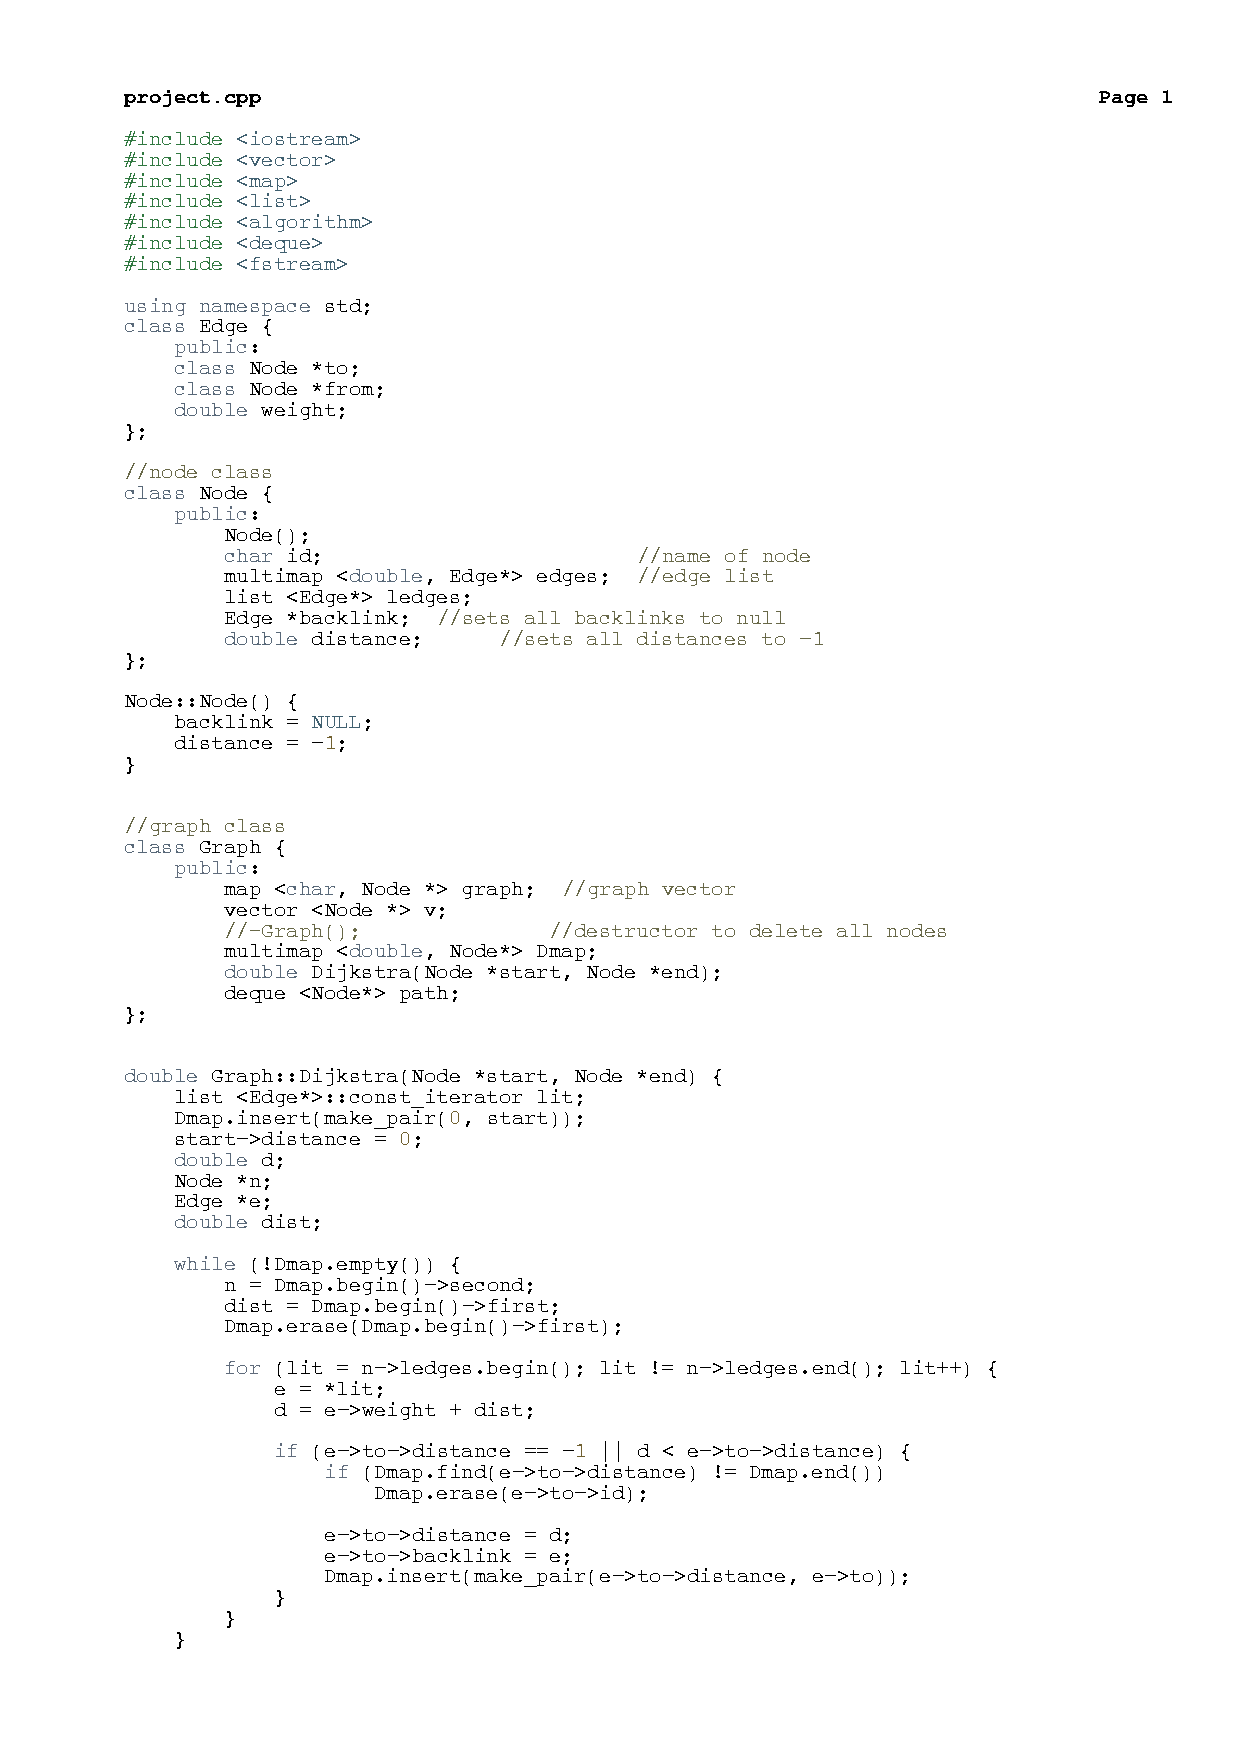
\includepdf[pages=-]{Noah Program 6 1.pdf}

% \subsection{Discussion}
% discussion of the Program results -- if the Program actually gives fastest route!

\newpage
\section{Works Cited} 
Labeled Map of Knoxville Map is from Apple Maps \\
Data collected from Google Maps 

\newpage
\section{Latex/Python/etc Notes}
$\bullet$ To comment out code: command-/ \\
$\bullet$ Online Jupyter Notebook Viewer: \url{https://htmtopdf.herokuapp.com/ipynbviewer/}

\newpage
\section{Time Log}
\subsection{NOAH}
\subsubsection*{MAY}

 %5/23-5/29
\begin{tabular}{ |m{1cm}||m{1cm}|m{1cm}|m{1cm}|m{1cm}|m{1cm}|m{1cm}|m{1cm}||m{1cm}|} 
\hline
 & 5/23 & 5/24 & 5/25 & 5/26 & 5/27 & 5/28 & 5/29 & \\ 
\hline
\rowcolor{lightgray}
\cellcolor{white} & Mon & Tue & Wed & Thu & Fri & Sat & Sun & \cellcolor{white}\\ 
\hline
\hline
 & & & & & 9:00 & & 3:30 & \\ 
\hline
 & & & & & 10:00 & & 7:00 & \\ 
\hline
 & & & & & & & & \\ 
\hline
 & & & & & 8:00 & & & \\ 
\hline
 & & & & & 11:00 & & & \\ 
\hline
\textbf{Total:} & 0:00 & 0:00 & 0:00 & 0:00 & 4:00 & 0:00 & 3:30 & \textbf{7:30} \\
\hline
\end{tabular}
\flushleft
\subsubsection*{JUNE}

 %5/30-6/5
\begin{tabular}{ |m{1cm}||m{1cm}|m{1cm}|m{1cm}|m{1cm}|m{1cm}|m{1cm}|m{1cm}||m{1cm}|} 
\hline
 & 5/30 & 5/31 & 6/1 & 6/2 & 6/3 & 6/4 & 6/5 & \\ 
\hline
\rowcolor{lightgray} 
\cellcolor{white} & Mon & Tue & Wed & Thu & Fri & Sat & Sun & \cellcolor{white}\\ 
\hline
\hline
 & 12:30 & & 5:30 & & & & & \\ 
\hline
 & 2:30 & & 8:30 & & & & & \\ 
\hline
 & & & & & & & & \\ 
\hline
 & & & & & & & & \\ 
\hline
 & & & & & & & & \\ 
\hline
\textbf{Total:} & 2:00 & 0:00 & 3:00 & 0:00 & 0:00 & 0:00 & 0:00 & \textbf{5:00} \\
\hline
\end{tabular}

\vspace{0.2in}

 %6/6-6/12
\begin{tabular}{ |m{1cm}||m{1cm}|m{1cm}|m{1cm}|m{1cm}|m{1cm}|m{1cm}|m{1cm}||m{1cm}|} 
\hline
 & 6/6 & 6/7 & 6/8 & 6/9 & 6/10 & 6/11 & 6/12 & \\ 
\hline
\rowcolor{lightgray} 
\cellcolor{white} & Mon & Tue & Wed & Thu & Fri & Sat & Sun & \cellcolor{white}\\ 
\hline
\hline
 & & & &10:00 & & & & \\ 
\hline
 & & & &10:30 & & & & \\ 
\hline
 & & & & & & & & \\ 
\hline
 & & & & & & & & \\ 
\hline
 & & & & & & & & \\ 
\hline
\textbf{Total:} & 0:00 & 0:00 & 0:00 & 0:00 & 0:00 & 0:00 & 0:00 & \textbf{0:00} \\
\hline
\end{tabular}

\vspace{0.2in}

 %6/13-6/19
\begin{tabular}{ |m{1cm}||m{1cm}|m{1cm}|m{1cm}|m{1cm}|m{1cm}|m{1cm}|m{1cm}||m{1cm}|} 
\hline
\textsc{Week 1} & 6/13 & 6/14 & 6/15 & 6/16 & 6/17 & 6/18 & 6/19 & \\ 
\hline
\rowcolor{lightgray} 
\cellcolor{white} & Mon & Tue & Wed & Thu & Fri & Sat & Sun & \cellcolor{white}\\ 
\hline
\hline
 & & & 6:00 & & & & & \\ 
\hline
 & & & 9:30 & & & & & \\ 
\hline
 & & & & & & & & \\ 
\hline
 & & & & & & & & \\ 
\hline
 & & & & & & & & \\ 
\hline
\textbf{Total:} & 0:00 & 0:00 & 3:30 & 0:00 & 0:00 & 0:00 & 0:00 & \textbf{3:30} \\
\hline
\end{tabular}

\vspace{0.2in}

 %6/20-6/26
\begin{tabular}{ |m{1cm}||m{1cm}|m{1cm}|m{1cm}|m{1cm}|m{1cm}|m{1cm}|m{1cm}||m{1cm}|} 
\hline
\textsc{Week 2} & 6/20 & 6/21 & 6/22 & 6/23 & 6/24 & 6/25 & 6/26 & \\ 
\hline
\rowcolor{lightgray} 
\cellcolor{white} & Mon & Tue & Wed & Thu & Fri & Sat & Sun & \cellcolor{white}\\ 
\hline
\hline
 & & & & & & & & \\ 
\hline
 & & & & & & & & \\ 
\hline
 & & & & & & & & \\ 
\hline
 & & & & & & & & \\ 
\hline
 & & & & & & & & \\ 
\hline
\textbf{Total:} & 0:00 & 0:00 & 0:00 & 0:00 & 0:00 & 0:00 & 0:00 & \textbf{0:00} \\
\hline
\end{tabular}

\vspace{0.2in}

 %6/27-7/3
\begin{tabular}{ |m{1cm}||m{1cm}|m{1cm}|m{1cm}|m{1cm}|m{1cm}|m{1cm}|m{1cm}||m{1cm}|} 
\hline
\textsc{Week 3} & 6/27 & 6/28 & 6/29 & 6/30 & 7/1 & 7/2 & 7/3 & \\ 
\hline
\rowcolor{lightgray} 
\cellcolor{white} & Mon & Tue & Wed & Thu & Fri & Sat & Sun & \cellcolor{white}\\ 
\hline
\hline
 & & & & & & & & \\ 
\hline
 & & & & & & & & \\ 
\hline
 & & & & & & & & \\ 
\hline
 & & & & & & & & \\ 
\hline
 & & & & & & & & \\ 
\hline
\textbf{Total:} & 0:00 & 0:00 & 0:00 & 0:00 & 0:00 & 0:00 & 0:00 & \textbf{0:00} \\
\hline
\end{tabular}

\flushleft\subsubsection*{JULY}

 %7/4-7/10
\begin{tabular}{ |m{1cm}||m{1cm}|m{1cm}|m{1cm}|m{1cm}|m{1cm}|m{1cm}|m{1cm}||m{1cm}|} 
\hline
\textsc{Week 4} & 7/4 & 7/5 & 7/6 & 7/7 & 7/8 & 7/9 & 7/10 & \\ 
\hline
\rowcolor{lightgray} 
\cellcolor{white} & Mon & Tue & Wed & Thu & Fri & Sat & Sun & \cellcolor{white}\\ 
\hline
\hline
 & & & & & & & & \\ 
\hline
 & & & & & & & & \\ 
\hline
 & & & & & & & & \\ 
\hline
 & & & & & & & & \\ 
\hline
 & & & & & & & & \\ 
\hline
\textbf{Total:} & 0:00 & 0:00 & 0:00 & 0:00 & 0:00 & 0:00 & 0:00 & \textbf{0:00} \\
\hline
\end{tabular}

\vspace{0.1in}
\flushleft
 %7/11-7/17
\begin{tabular}{ |m{1cm}||m{1cm}|m{1cm}|m{1cm}|m{1cm}|m{1cm}|m{1cm}|m{1cm}||m{1cm}|} 
\hline
\textsc{Week 5} & 7/11 & 7/12 & 7/13 & 7/14 & 7/15 & 7/16 & 7/17 & \\ 
\hline
\rowcolor{lightgray} 
\cellcolor{white} & Mon & Tue & Wed & Thu & Fri & Sat & Sun & \cellcolor{white}\\ 
\hline
\hline
 & & & & & & & & \\ 
\hline
 & & & & & & & & \\ 
\hline
 & & & & & & & & \\ 
\hline
 & & & & & & & & \\ 
\hline
 & & & & & & & & \\ 
\hline
\textbf{Total:} & 0:00 & 0:00 & 0:00 & 0:00 & 0:00 & 0:00 & 0:00 & \textbf{0:00} \\
\hline
\end{tabular}

\vspace{0.2in}

 %7/18-7/24
\begin{tabular}{ |m{1cm}||m{1cm}|m{1cm}|m{1cm}|m{1cm}|m{1cm}|m{1cm}|m{1cm}||m{1cm}|} 
\hline
\textsc{Week 6} & 7/18 & 7/19 & 7/20 & 7/21 & 7/22 & 7/23 & 7/24 & \\ 
\hline
\rowcolor{lightgray} 
\cellcolor{white} & Mon & Tue & Wed & Thu & Fri & Sat & Sun & \cellcolor{white}\\ 
\hline
\hline
 & & & & & & & & \\ 
\hline
 & & & & & & & & \\ 
\hline
 & & & & & & & & \\ 
\hline
 & & & & & & & & \\ 
\hline
 & & & & & & & & \\ 
\hline
\textbf{Total:} & 0:00 & 0:00 & 0:00 & 0:00 & 0:00 & 0:00 & 0:00 & \textbf{0:00} \\
\hline
\end{tabular}

\vspace{0.2in}

 %7/25-7/31
\begin{tabular}{ |m{1cm}||m{1cm}|m{1cm}|m{1cm}|m{1cm}|m{1cm}|m{1cm}|m{1cm}||m{1cm}|} 
\hline
\textsc{Week 7} & 7/25 & 7/26 & 7/27 & 7/28 & 7/29 & 7/30 & 7/31 & \\ 
\hline
\rowcolor{lightgray} 
\cellcolor{white} & Mon & Tue & Wed & Thu & Fri & Sat & Sun & \cellcolor{white}\\ 
\hline
\hline
 & & & & & & & & \\ 
\hline
 & & & & & & & & \\ 
\hline
 & & & & & & & & \\ 
\hline
 & & & & & & & & \\ 
\hline
 & & & & & & & & \\ 
\hline
\textbf{Total:} & 0:00 & 0:00 & 0:00 & 0:00 & 0:00 & 0:00 & 0:00 & \textbf{0:00} \\
\hline
\end{tabular}


\flushleft
\subsubsection*{AUGUST}

 %8/1-8/7
\begin{tabular}{ |m{1cm}||m{1cm}|m{1cm}|m{1cm}|m{1cm}|m{1cm}|m{1cm}|m{1cm}||m{1cm}|} 
\hline
\textsc{Week 8} & 8/1& 8/2 & 8/3 & 8/4 & 8/5 & 8/6 & 8/7 & \\ 
\hline
\rowcolor{lightgray} 
\cellcolor{white} & Mon & Tue & Wed & Thu & Fri & Sat & Sun & \cellcolor{white}\\ 
\hline
\hline
 & & & & & & & & \\ 
\hline
 & & & & & & & & \\ 
\hline
 & & & & & & & & \\ 
\hline
 & & & & & & & & \\ 
\hline
 & & & & & & & & \\ 
\hline
\textbf{Total:} & 0:00 & 0:00 & 0:00 & 0:00 & 0:00 & 0:00 & 0:00 & \textbf{0:00} \\
\hline
\end{tabular}

\vspace{0.2in}

 %8/8-8/14
\begin{tabular}{ |m{1cm}||m{1cm}|m{1cm}|m{1cm}|m{1cm}|m{1cm}|m{1cm}|m{1cm}||m{1cm}|} 
\hline
\textsc{Week 9} & 8/8& 8/9 & 8/10 & 8/11 & 8/12 & 8/13 & 8/14 & \\ 
\hline
\rowcolor{lightgray} 
\cellcolor{white} & Mon & Tue & Wed & Thu & Fri & Sat & Sun & \cellcolor{white}\\ 
\hline
\hline
 & & & & & & & & \\ 
\hline
 & & & & & & & & \\ 
\hline
 & & & & & & & & \\ 
\hline
 & & & & & & & & \\ 
\hline
 & & & & & & & & \\ 
\hline
\textbf{Total:} & 0:00 & 0:00 & 0:00 & 0:00 & 0:00 & 0:00 & 0:00 & \textbf{0:00} \\
\hline
\end{tabular}

\vspace{0.2in}

 %8/15-8/21
\begin{tabular}{ |m{1cm}||m{1cm}|m{1cm}|m{1cm}|m{1cm}|m{1cm}|m{1cm}|m{1cm}||m{1cm}|} 
\hline
\textsc{Week 10} & 8/15 & 8/16 & 8/17 & 8/18 & 8/19 & 8/20 & 8/21 & \\ 
\hline
\rowcolor{lightgray} 
\cellcolor{white} & Mon & Tue & Wed & Thu & Fri & Sat & Sun & \cellcolor{white}\\ 
\hline
\hline
 & & & & & & & & \\ 
\hline
 & & & & & & & & \\ 
\hline
 & & & & & & & & \\ 
\hline
 & & & & & & & & \\ 
\hline
 & & & & & & & & \\ 
\hline
\textbf{Total:} & 0:00 & 0:00 & 0:00 & 0:00 & 0:00 & 0:00 & 0:00 & \textbf{0:00} \\
\hline
\end{tabular}

\newpage

\subsection{KRISTINA} 

\subsubsection*{MAY} 
\\
 %5/23-5/29
\begin{tabular}{ |m{1cm}||m{1cm}|m{1cm}|m{1cm}|m{1cm}|m{1cm}|m{1cm}|m{1cm}||m{1cm}|} 
\hline
 & 5/23 & 5/24 & 5/25 & 5/26 & 5/27 & 5/28 & 5/29 & \\ 
\hline
\rowcolor{lightgray} 
\cellcolor{white} & Mon & Tue & Wed & Thu & Fri & Sat & Sun & \cellcolor{white}\\ 
\hline
\hline
 & & & & & 9:00 & & 3:30 & \\ 
\hline
 & & & & & 11:00 & & 7:00 & \\ 
\hline
 & & & & & & & & \\ 
\hline
 & & & & & 6:00 & & & \\ 
\hline
 & & & & & 6:30 & & & \\ 
\hline
 & & & & & & & & \\
\hline
\textbf{Total:} & 0:00 & 0:00 & 0:00 & 0:00 & 2:30 & 0:00 & 3:30 & \textbf{6:00} \\
\hline
\end{tabular} \\

\vspace{0.2in}

\subsubsection*{JUNE} 
 %5/30-6/5
\begin{tabular}{ |m{1cm}||m{1cm}|m{1cm}|m{1cm}|m{1cm}|m{1cm}|m{1cm}|m{1cm}||m{1cm}|} 
\hline
 & 5/30 & 5/31 & 6/1 & 6/2 & 6/3 & 6/4 & 6/5 & \\ 
\hline
\rowcolor{lightgray} 
\cellcolor{white} & Mon & Tue & Wed & Thu & Fri & Sat & Sun & \cellcolor{white}\\ 
\hline
\hline
 & 5:00 & & 2:00 & & 9:30 & & 9:00 & \\ 
\hline
 & 7:00 & & 7:00 & & 11:30 & & 10:00 & \\ 
\hline
 & & & & & & & & \\ 
\hline
 & & & & & & & & \\ 
\hline
 & & & & & & & & \\ 
\hline
\textbf{Total:} & 2:00 & 0:00 & 5:00 & 0:00 & 2:00 & 0:00 & 1:00 & \textbf{10:00} \\
\hline
\end{tabular} 

\vspace{0.2in}

 %6/6-6/12
\begin{tabular}{ |m{1cm}||m{1cm}|m{1cm}|m{1cm}|m{1cm}|m{1cm}|m{1cm}|m{1cm}||m{1cm}|} 
\hline
 & 6/6 & 6/7 & 6/8 & 6/9 & 6/10 & 6/11 & 6/12 & \\ 
\hline
\rowcolor{lightgray} 
\cellcolor{white} & Mon & Tue & Wed & Thu & Fri & Sat & Sun & \cellcolor{white}\\ 
\hline
\hline
 & & & & 10:00 & 10:00 & & & \\ 
\hline
 & & & & 10:30 & 12:00 & & & \\ 
\hline
 & & & & & & & & \\ 
\hline
 & & & & 9:00 & 2:00 & & & \\ 
\hline
 & & & & 10:30 & 5:00 & & & \\ 
\hline
& & & & & & & & \\
\hline
& & & & & 7:00 & & & \\
\hline
& & & & & 10:00 & & & \\
\hline
& & & & & & & & \\
\hline
\textbf{Total:} & 0:00 & 0:00 & 0:00 & 2:00 & 8:00 & 0:00 & 0:00 & \textbf{10:00} \\
\hline
\end{tabular}

\vspace{0.2in}

%6/13-6/19
\begin{tabular}{ |m{1cm}||m{1cm}|m{1cm}|m{1cm}|m{1cm}|m{1cm}|m{1cm}|m{1cm}||m{1cm}|} 
\hline
\textsc{Week 1} & 6/13 & 6/14 & 6/15 & 6/16 & 6/17 & 6/18 & 6/19 & \\ 
\hline
\rowcolor{lightgray} 
\cellcolor{white} & Mon & Tue & Wed & Thu & Fri & Sat & Sun & \cellcolor{white}\\ 
\hline
\hline
 & & & 6:00 & & & & & \\ 
\hline
 & & & 9:30 & & & & & \\ 
\hline
 & & & & & & & & \\ 
\hline
 & & & & & & & & \\ 
\hline
 & & & & & & & & \\ 
\hline
\textbf{Total:} & 0:00 & 0:00 & 3:30 & 0:00 & 0:00 & 0:00 & 0:00 & \textbf{3:30} \\
\hline
\end{tabular}

\vspace{0.2in}

 %6/20-6/26
\begin{tabular}{ |m{1cm}||m{1cm}|m{1cm}|m{1cm}|m{1cm}|m{1cm}|m{1cm}|m{1cm}||m{1cm}|} 
\hline
\textsc{Week 2} & 6/20 & 6/21 & 6/22 & 6/23 & 6/24 & 6/25 & 6/26 & \\ 
\hline
\rowcolor{lightgray} 
\cellcolor{white} & Mon & Tue & Wed & Thu & Fri & Sat & Sun & \cellcolor{white}\\ 
\hline
\hline
 & & & & & & & & \\ 
\hline
 & & & & & & & & \\ 
\hline
 & & & & & & & & \\ 
\hline
 & & & & & & & & \\ 
\hline
 & & & & & & & & \\ 
\hline
\textbf{Total:} & 0:00 & 0:00 & 0:00 & 0:00 & 0:00 & 0:00 & 0:00 & \textbf{0:00} \\
\hline
\end{tabular}

\vspace{0.2in}

 %6/27-7/3
\begin{tabular}{ |m{1cm}||m{1cm}|m{1cm}|m{1cm}|m{1cm}|m{1cm}|m{1cm}|m{1cm}||m{1cm}|} 
\hline
\textsc{Week 3} & 6/27 & 6/28 & 6/29 & 6/30 & 7/1 & 7/2 & 7/3 & \\ 
\hline
\rowcolor{lightgray} 
\cellcolor{white} & Mon & Tue & Wed & Thu & Fri & Sat & Sun & \cellcolor{white}\\ 
\hline
\hline
 & & & & & & & & \\ 
\hline
 & & & & & & & & \\ 
\hline
 & & & & & & & & \\ 
\hline
 & & & & & & & & \\ 
\hline
 & & & & & & & & \\ 
\hline
\textbf{Total:} & 0:00 & 0:00 & 0:00 & 0:00 & 0:00 & 0:00 & 0:00 & \textbf{0:00} \\
\hline
\end{tabular}

\vspace{0.2in}

\subsubsection*{JULY}

 %7/4-7/10
\begin{tabular}{ |m{1cm}||m{1cm}|m{1cm}|m{1cm}|m{1cm}|m{1cm}|m{1cm}|m{1cm}||m{1cm}|} 
\hline
\textsc{Week 4} & 7/4 & 7/5 & 7/6 & 7/7 & 7/8 & 7/9 & 7/10 & \\ 
\hline
\rowcolor{lightgray} 
\cellcolor{white} & Mon & Tue & Wed & Thu & Fri & Sat & Sun & \cellcolor{white}\\ 
\hline
\hline
 & & & & & & & & \\ 
\hline
 & & & & & & & & \\ 
\hline
 & & & & & & & & \\ 
\hline
 & & & & & & & & \\ 
\hline
 & & & & & & & & \\ 
\hline
\textbf{Total:} & 0:00 & 0:00 & 0:00 & 0:00 & 0:00 & 0:00 & 0:00 & \textbf{0:00} \\
\hline
\end{tabular}

\vspace{0.2in}

 %7/11-7/17
\begin{tabular}{ |m{1cm}||m{1cm}|m{1cm}|m{1cm}|m{1cm}|m{1cm}|m{1cm}|m{1cm}||m{1cm}|} 
\hline
\textsc{Week 5} & 7/11 & 7/12 & 7/13 & 7/14 & 7/15 & 7/16 & 7/17 & \\ 
\hline
\rowcolor{lightgray} 
\cellcolor{white} & Mon & Tue & Wed & Thu & Fri & Sat & Sun & \cellcolor{white}\\ 
\hline
\hline
 & & & & & & & & \\ 
\hline
 & & & & & & & & \\ 
\hline
 & & & & & & & & \\ 
\hline
 & & & & & & & & \\ 
\hline
 & & & & & & & & \\ 
\hline
\textbf{Total:} & 0:00 & 0:00 & 0:00 & 0:00 & 0:00 & 0:00 & 0:00 & \textbf{0:00} \\
\hline
\end{tabular}

\vspace{0.2in}

%7/18-7/24
\begin{tabular}{ |m{1cm}||m{1cm}|m{1cm}|m{1cm}|m{1cm}|m{1cm}|m{1cm}|m{1cm}||m{1cm}|} 
\hline
\textsc{Week 6} & 7/18 & 7/19 & 7/20 & 7/21 & 7/22 & 7/23 & 7/24 & \\ 
\hline
\rowcolor{lightgray} 
\cellcolor{white} & Mon & Tue & Wed & Thu & Fri & Sat & Sun & \cellcolor{white}\\ 
\hline
\hline
 & & & & & & & & \\ 
\hline
 & & & & & & & & \\ 
\hline
 & & & & & & & & \\ 
\hline
 & & & & & & & & \\ 
\hline
 & & & & & & & & \\ 
\hline
\textbf{Total:} & 0:00 & 0:00 & 0:00 & 0:00 & 0:00 & 0:00 & 0:00 & \textbf{0:00} \\
\hline
\end{tabular}

\vspace{0.2in}

 %7/25-7/31
\begin{tabular}{ |m{1cm}||m{1cm}|m{1cm}|m{1cm}|m{1cm}|m{1cm}|m{1cm}|m{1cm}||m{1cm}|} 
\hline
\textsc{Week 7} & 7/25 & 7/26 & 7/27 & 7/28 & 7/29 & 7/30 & 7/31 & \\ 
\hline
\rowcolor{lightgray} 
\cellcolor{white} & Mon & Tue & Wed & Thu & Fri & Sat & Sun & \cellcolor{white}\\ 
\hline
\hline
 & & & & & & & & \\ 
\hline
 & & & & & & & & \\ 
\hline
 & & & & & & & & \\ 
\hline
 & & & & & & & & \\ 
\hline
 & & & & & & & & \\ 
\hline
\textbf{Total:} & 0:00 & 0:00 & 0:00 & 0:00 & 0:00 & 0:00 & 0:00 & \textbf{0:00} \\
\hline
\end{tabular}

\subsubsection*{AUGUST}

 %8/1-8/7
\begin{tabular}{ |m{1cm}||m{1cm}|m{1cm}|m{1cm}|m{1cm}|m{1cm}|m{1cm}|m{1cm}||m{1cm}|} 
\hline
\textsc{Week 8} & 8/1& 8/2 & 8/3 & 8/4 & 8/5 & 8/6 & 8/7 & \\ 
\hline
\rowcolor{lightgray} 
\cellcolor{white} & Mon & Tue & Wed & Thu & Fri & Sat & Sun & \cellcolor{white}\\ 
\hline
\hline
 & & & & & & & & \\ 
\hline
 & & & & & & & & \\ 
\hline
 & & & & & & & & \\ 
\hline
 & & & & & & & & \\ 
\hline
 & & & & & & & & \\ 
\hline
\textbf{Total:} & 0:00 & 0:00 & 0:00 & 0:00 & 0:00 & 0:00 & 0:00 & \textbf{0:00} \\
\hline
\end{tabular}

\vspace{0.2in}

 %8/8-8/14
\begin{tabular}{ |m{1cm}||m{1cm}|m{1cm}|m{1cm}|m{1cm}|m{1cm}|m{1cm}|m{1cm}||m{1cm}|} 
\hline
\textsc{Week 9} & 8/8& 8/9 & 8/10 & 8/11 & 8/12 & 8/13 & 8/14 & \\ 
\hline
\rowcolor{lightgray} 
\cellcolor{white} & Mon & Tue & Wed & Thu & Fri & Sat & Sun & \cellcolor{white}\\ 
\hline
\hline
 & & & & & & & & \\ 
\hline
 & & & & & & & & \\ 
\hline
 & & & & & & & & \\ 
\hline
 & & & & & & & & \\ 
\hline
 & & & & & & & & \\ 
\hline
\textbf{Total:} & 0:00 & 0:00 & 0:00 & 0:00 & 0:00 & 0:00 & 0:00 & \textbf{0:00} \\
\hline
\end{tabular}

\vspace{0.2in}

 %8/15-8/21
\begin{tabular}{ |m{1cm}||m{1cm}|m{1cm}|m{1cm}|m{1cm}|m{1cm}|m{1cm}|m{1cm}||m{1cm}|} 
\hline
\textsc{Week 10} & 8/15 & 8/16 & 8/17 & 8/18 & 8/19 & 8/20 & 8/21 & \\ 
\hline
\rowcolor{lightgray} 
\cellcolor{white} & Mon & Tue & Wed & Thu & Fri & Sat & Sun & \cellcolor{white}\\ 
\hline
\hline
 & & & & & & & & \\ 
\hline
 & & & & & & & & \\ 
\hline
 & & & & & & & & \\ 
\hline
 & & & & & & & & \\ 
\hline
 & & & & & & & & \\ 
\hline
\textbf{Total:} & 0:00 & 0:00 & 0:00 & 0:00 & 0:00 & 0:00 & 0:00 & \textbf{0:00} \\
\hline
\end{tabular}

\end{document}
